\section{Préambule : une suite de benchmarks pour OpenMP~4.0, les KASTORS}

\subsection{Motivation pour une nouvelle suite de benchmarks}

Le support pour les applications à base de flots de données dans OpenMP est arrivé avec la version 4.0, qui est sortie au démarrage de cette thèse.
Nous n'avions donc pas d'applications de référence pour utiliser les fonctionnalités ajoutées dans OpenMP, et nous avons donc décidé d'introduire une suite de benchmarks - les KASTORS~\cite{Virouleau2014} - spécifiquement orientée vers ces fonctionnalités, en étendant et regroupant certaines applications existantes.

Il existe évidemment plusieurs suites de benchmarks à destination des architectures à mémoire partagée : d'une part pour les applications à base de tâches indépendantes et utilisant OpenMP~3.0, et d'autre part pour les applications à base de flots de données, mais écrites dans des langages différents.

Parmi les benchmarks populaire ciblant spécifiquement OpenMP, on peut citer la Barcelona OpenMP Task Suite~\cite{Duran2009} (BOTS), proposant des applications à base de tâches OpenMP~3.0 afin d'évaluer le comportement d'OpenMP en fonction de la manière de générer les tâches et de la répartition de la charge de travail.
Nous avons d'ailleurs adapté certaines de leurs applications - SparseLU et Strassen - dans les KASTORS, dont nous parlons plus en détails dans les sections~\ref{sec:kastors:sparselu} et~\ref{sec:kastors:strassen}

Parmi les benchmarks ciblant des modèles de programmations à base de tâche avec dépendances, on peut principalement nommer les PLASMA~\cite{Kurzak2013}.
Cette bibliothèque développée à ICL/UTK met à disposition un grand nombre d'algorithmes d'algèbre linéaire dense, optimisés pour les architectures multi-coeurs.

Nous avions donc assez d'éléments de base pour construire un ensemble d'applications, avec en tête les objectifs suivant :
\begin{itemize}
  \item Rassembler et proposer une suite d'applications exploitant les dépendances introduites avec OpenMP~4.0
  \item Comparer la version utilisant des flots de données à la version utilisant des synchronisations explicites. Le but étant de montrer que le support exécutif peut gérer les synchronisations plus finement, et par conséquent améliorer les performances sans changer l'algorithme.
  \item Avoir une base adaptée pour développer les extensions présentées dans les sections~\ref{sec:openmp:langage} et~\ref{sec:openmp:runtime}.
\end{itemize}

Les sections suivantes décrivent les différents applications de la suite : d'où ils viennent, comment nous les avons étendu pour utiliser les dépendances de données, ainsi que comment nous les avons intégrés.


\subsection{Description des applications}

Les applications suivantes proviennent de différentes suites de benchmarks, et ont été modifiées afin d'utiliser les dépendances de données plutôt que d'autres moyen de synchronisation.

\subsubsection{Factorisations de Cholesky, QR, et LU}

Ces trois applications ont été adaptées des PLASMA.
Dans les PLASMA plusieurs implémentations de chaque algorithme sont disponibles, utilisant soit un ordonnancement statique, soit un ordonnancement dynamique.
Les algorithmes à ordonnancement dynamique sont construit sur le support exécutif QUARK~\cite{YarKhan2011}, qui utilise un modèle avec dépendances de données pour ordonnancer les tâches.

Les trois algorithmes que nous avons sélectionné sont les factorisations de Cholesky, QR, et LU, respectivement nommés DPOTRF, DGEQRF, et DGETRF dans PLASMA.
Ils opèrent tous sur des matrices de nombres flottant à double précision (type |double|).

L'implémentation initiale utilise plusieurs niveaux de wrappers, avec packing et unpacking de paramètres à chaque niveau, ce qui affecte la lisibilité du code et augmente grandement le risque d'erreur.

Les listings~\ref{lst:kastors:dyn} et~\ref{lst:kastors:dyn-omp} montrent respectivement la version dynamique originale, et les transformation que l'on a fait pour porter le code en OpenMP~4.0.
Dans la version originale, la function |wrapper_blas_function| effectue l'unpacking des paramètres avant d'appeler la vraie fonction BLAS/LAPACK sur laquelle elle est construite.
La transformation en OpenMP~4.0 a donné lieu au retrait de plusieurs niveau d'encapsulation, ce qui facilite la lecture du code, la maintenabilité du code, et enlève le besoin de gérer ces paramètres.

\begin{lstlisting}[caption=Format de l'algorithme dynamique,label=lst:kastors:dyn]
wrapper_algorithm_dynamic_call(...) {
  // code séquentiel
  for (...)
    QUARK_Insert_Task(wrapper_blas_function, packed_parameters);
  // code séquentiel
  for (...)
    QUARK_Insert_Task(
        wrapper_another_blas_function,
        packed_parameters);
  // code sequentiel
}
\end{lstlisting}
\begin{lstlisting}[caption=Format de l'algorithme OpenMP,label=lst:kastors:dyn-omp]
algorithm_call(...) {
    // code séquentiel
    for (...)
#pragma omp task depend(inout:array[...])
        blas_function(...);
    // code séquentiel
    for (...)
#pragma omp task depend(inout:array[...])
        another_blas_function(...);
    // code séquentiel
}
\end{lstlisting}


\subsubsection{Jacobi}

C'est un algorithme de type Stencil : c'est un algorithme itératif, et à chaque itérations les différents éléments d'un tableau sont mis à jour en suivant la même formules dépendant généralement des éléments voisins.

En pratique cet algorithme résout l'équation de Poisson sur le carré unitaire [0,1]x[0,1], qui est divisé en une grille de NxN points espacés régulièrement.
Le noyau de calcul principal est un Stencil à 5 points, en 2 dimensions.
Ce noyau est appliqué successivement jusqu'à ce qu'une convergence soit détectée.

Nous avons implémenté deux versions bloquées de ce noyau, en utilisant d'une part des tâches sans dépendances, et d'autre part des tâches avec dépendances.

\subsubsection{SparseLU}\label{sec:kastors:sparselu}

Cette application calcule la factorisation LU d'une matrice creuse.
Nous avons modifié l'implémentation originale des BOTS pour ajouter des dépendances de données.
Ces modifications sont décrites dans les listings~\ref{lst:kastors:sparseLU} et~\ref{lst:kastors:sparseLU-deps}.

\begin{lstlisting}[caption=LU utilisant des tâches indépendantes,label=lst:kastors:sparseLU]
for (k=0; k<NB; k++) {
  lu0(M[k*NB+k]);
  for (j=k+1; j<NB; j++)
#pragma omp task untied shared(M)
    fwd(M[k*NB+k], M[k*NB+j]);

  for (i=k+1; i<NB; i++)
#pragma omp task untied shared(M)
    bdiv(M[k*NB+k], M[i*NB+k]);

#pragma omp taskwait

  for (i=k+1; i<NB; i++)
    for (j=k+1; j<NB; j++)
#pragma omp task untied shared(M)
      bmod(M[i*NB+k],
           M[k*NB+j],
           M[i*NB+j]);
#pragma omp taskwait
}
\end{lstlisting}

\begin{lstlisting}[caption=LU utilisant des tâches avec dépendances,label=lst:kastors:sparseLU-deps]
for (k=0; k<NB; k++) {
#pragma omp task untied shared(M)\
    depend(inout: M[k*NB+k:BS*BS])
  lu0(M[k*NB+k]);
  for (j=k+1; j<NB; j++)
#pragma omp task untied shared(M)\
    depend(in: M[k*NB+k:BS*BS])\
    depend(inout: M[k*NB+j:BS*BS])
    fwd(M[k*NB+k], M[k*NB+j]);

  for (i=k+1; i<NB; i++)
#pragma omp task untied shared(M)\
    depend(in: M[k*NB+k:BS*BS])\
    depend(inout: M[i*NB+k:BS*BS])
    bdiv(M[k*NB+k], M[i*NB+k]);

  for (i=k+1; i<NB; i++)
    for (j=k+1; j<NB; j++)
#pragma omp task untied shared(M)\
   depend(in: M[i*NB+k:BS*BS])\
   depend(in: M[k*NB+j:BS*BS])\
   depend(inout: M[i*NB+j:BS*BS])
    bmod(M[i*NB+k],M[k*NB+j],M[i*NB+j]);
}
\end{lstlisting}

\subsubsection{Strassen}\label{sec:kastors:strassen}

L'application Strassen utilise des décompositions de matrices pour calculer le produit de grandes matrices denses.
De manière similaire à SparseLU, nous avons modifié l'implémentation des BOTS pour ajouter du parallélisme au niveau des additions dans l'algorithme, et nous avons exprimé des dépendances de données plutôt que d'utiliser une synchronisation à base de |taskwait|.

\subsection{Discussions et perspectives}

Nous avons évalué l'intérêt des tâches avec dépendances comparé aux tâches indépendantes dans l'article publié à IWOMP2014~\cite{Virouleau2014}.
Les expériences ont été mené sur toutes les applications avec plusieurs supports exécutifs.
Les résultats ont montrés que l'utilisation des dépendances n'était jamais négatif pour les performances, et induisait en fait une amélioration dans la majorité des cas que nous avons testé.
Cela a pu confirmer que les supports exécutifs pouvaient gérer les synchronisations finement, éliminant ainsi les inactivités des threads dues aux |taskwait|.

D'autres part, ces applications et expériences ont permises de mettre en évidence d'autres limitations des tâches OpenMP.

\begin{figure}[ht]
  \centering
  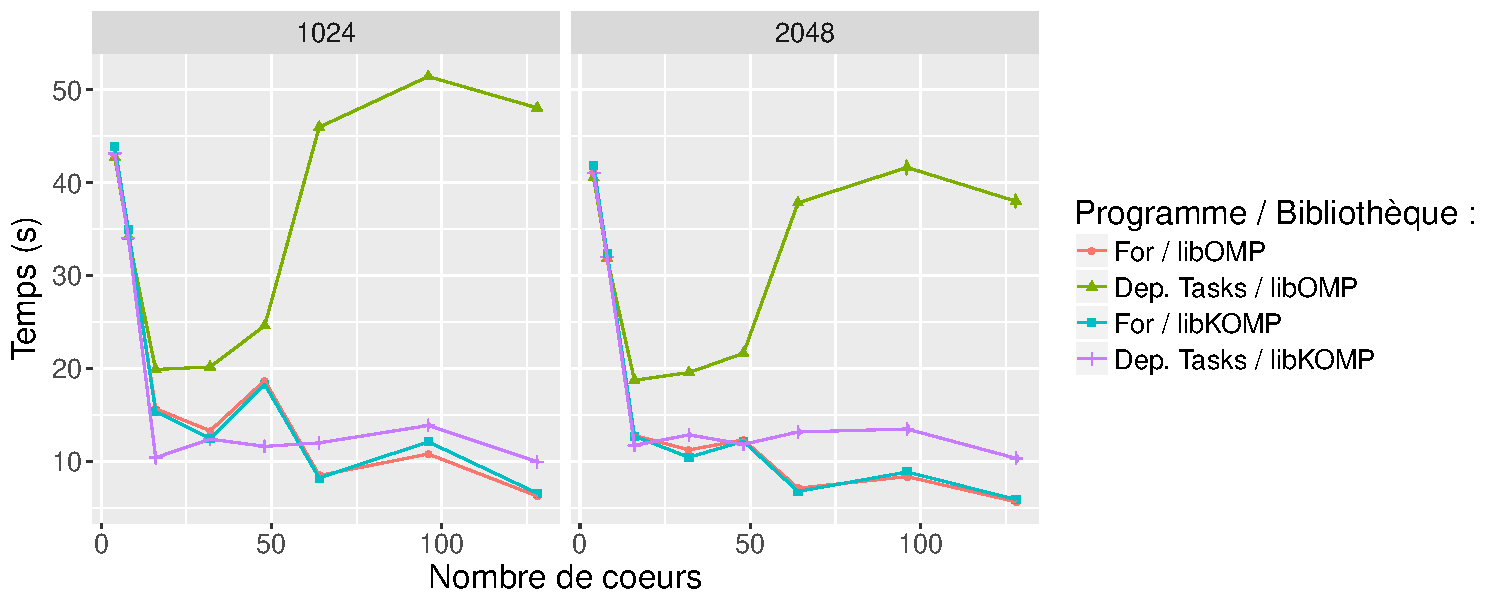
\includegraphics[width=\textwidth]{jacobi_scale_noaff}
  \caption{Comparaison des performances de Jacobi, avec une taille de matrice de 49152}\label{fig:contribs:openmp:kastors:jacobi-motiv}
\end{figure}

La figure~\ref{fig:contribs:openmp:kastors:jacobi-motiv} regroupe une comparaison de l'application de jacobi en fonction de la version implémentée (à base de boucles ou de tâche avec dépendances) et du support exécutif.
La scalabilité de l'application en elle même est limitée, mais il n'y a pas de raison, a priori, qu'il y ait une dégradation de performances de l'application avec l'augmentation du nombre de cœurs.
Jacobi est une application stencil, et chacune des tâches successives (ou groupe d'itérations pour la version à base de boucles) dépend énormément de la réutilisation du cache L2~: la structure de tâches ne permet pas d'exprimer ce genre de <<dépendances>>, lors de l'ordonnancement certaines tâches vont se faire voler et briser la localité du cache L2, introduisant une grosse dégradation des performances.

Ce problème pourrait être résolu si l'on pouvait exprimer une \emph{affinité} entre une tâche et un cœur de la machine, par exemple.
De plus les résultats de la section~\ref{sec:contribs:apps:cholesky:carton} ont montrés l'importance de la proximité des données pour les différents noyaux de Cholesky, ce qui représente une autre motivation pour la proposition d'une clause permettant l'expression d'une \emph{affinité} entre une tâche et un élément de la machine.

La section suivante aborde ce point, et la section~\ref{sec:contribs:perf_eval} décrit les résultats obtenus à partir des KASTORS étendus avec nos propositions.

